\part{The Basic Layer}

{\Large \emph{by Till Tantau}}


\bigskip
\noindent
\vskip1cm
\begin{codeexample}[graphic=white]
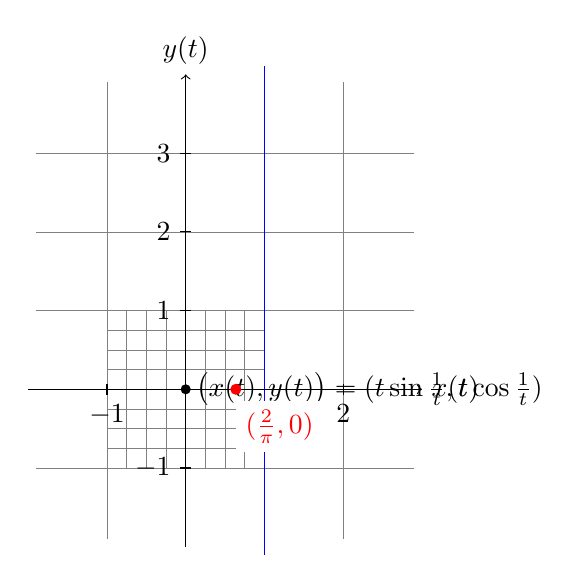
\begin{tikzpicture}
  \draw[gray,very thin] (-1.9,-1.9) grid (2.9,3.9)
          [step=0.25cm] (-1,-1) grid (1,1);
  \draw[blue] (1,-2.1) -- (1,4.1); % asymptote

  \draw[->] (-2,0) -- (3,0) node[right] {$x(t)$};
  \draw[->] (0,-2) -- (0,4) node[above] {$y(t)$};

  \foreach \pos in {-1,2}
    \draw[shift={(\pos,0)}] (0pt,2pt) -- (0pt,-2pt) node[below] {$\pos$};

  \foreach \pos in {-1,1,2,3}
    \draw[shift={(0,\pos)}] (2pt,0pt) -- (-2pt,0pt) node[left] {$\pos$};

  \fill (0,0) circle (0.064cm);
  \draw[thick,parametric,domain=0.4:1.5,samples=200]
    % The plot is reparameterised such that there are more samples
    % near the center.
    plot[id=asymptotic-example] function{(t*t*t)*sin(1/(t*t*t)),(t*t*t)*cos(1/(t*t*t))}
    node[right] {$\bigl(x(t),y(t)\bigr) = (t\sin \frac{1}{t}, t\cos \frac{1}{t})$};

  \fill[red] (0.63662,0) circle (2pt)
    node [below right,fill=white,yshift=-4pt] {$(\frac{2}{\pi},0)$};
\end{tikzpicture}
\end{codeexample}

\input{parts/The-Basic-Layer/sections/pgfmanual-zh-base-design}
\input{parts/The-Basic-Layer/sections/pgfmanual-zh-base-scopes}
\input{parts/The-Basic-Layer/sections/pgfmanual-zh-base-points}
\input{parts/The-Basic-Layer/sections/pgfmanual-zh-base-paths}
\input{parts/The-Basic-Layer/sections/pgfmanual-zh-base-decorations}
\input{parts/The-Basic-Layer/sections/pgfmanual-zh-base-actions}
\input{parts/The-Basic-Layer/sections/pgfmanual-zh-base-arrows}
\input{parts/The-Basic-Layer/sections/pgfmanual-zh-base-nodes}
\input{parts/The-Basic-Layer/sections/pgfmanual-zh-base-matrices}
\input{parts/The-Basic-Layer/sections/pgfmanual-zh-base-transformations}
\input{parts/The-Basic-Layer/sections/pgfmanual-zh-base-patterns}
\input{parts/The-Basic-Layer/sections/pgfmanual-zh-base-images}
\input{parts/The-Basic-Layer/sections/pgfmanual-zh-base-external}
\input{parts/The-Basic-Layer/sections/pgfmanual-zh-base-plots}
\input{parts/The-Basic-Layer/sections/pgfmanual-zh-base-layers}
\input{parts/The-Basic-Layer/sections/pgfmanual-zh-base-shadings}
\input{parts/The-Basic-Layer/sections/pgfmanual-zh-base-transparency}
\input{parts/The-Basic-Layer/sections/pgfmanual-zh-base-animations}
\input{parts/The-Basic-Layer/sections/pgfmanual-zh-base-internalregisters}
\input{parts/The-Basic-Layer/sections/pgfmanual-zh-base-quick}